

	\subsection{Конечные морфизмы и нормализация многообразия}

	\begin{theorem}\label{B_is_finite_A_module} 
		Пусть $L/K$~--- сепарабельное конечное расширение, $A \subset K$ и $K = \Frac(A)$. Пусть $B = \Int_{L}{A}$ и предположим, что $A$ нётерово и нормально\footnote{Кольцо называется нормальным, если любая его локализация в простом идеале целозамкнута. }. 

		Тогда $B$~--- конечнопорожденный $A$-модуль. 
	\end{theorem}
	\begin{proof}
		Это доказывается стандартным образом. Во-первых, из такой леммы из коммутативной алгебры следует, что $L = \Frac(B)$:

		\begin{lemma} 
			Пусть $Z$~--- дедекиндово кольцо с полем частных $Q$,  $F/Q$~--- конечное расширение, а $R = \Int_{F}{Z}$. Тогда $F = \Frac(R)$ и, следовательно, $R$ целозамкнуто. 
		\end{lemma}

		Теперь возьмём $\{ \omega_i \}_{i = 1}^{n}$~--- базис $L/K$, причём выберем $\omega_i \in B$. Рассмотрим билинейную форму следа 
		\[
			L \times L \to K, \quad (x, y) \mapsto \Tr(xy).
		\]

		Из курса теории полей известно, что так как расширение сепарабельно, эта форма невырожденна. Тогда возьмём двойственный базис к $\omega_i$, то есть рассмотрим такой набор $\{ \omega_i^* \}$, что 
		\[
			\Tr(\omega_i \omega_j^*) = \begin{cases} 1, & i = j \\ 0, & \text{ иначе. }\end{cases}
		\]
		Тогда мы имеем включения 
		\[
			A \omega_1 \oplus \ldots \oplus A \omega_n \subset B \subset A \omega_1^* \oplus \ldots \oplus A \omega_n^*. 
		\]
		Действительно, первое включение очевидно, докажем второе. Пусть $b = a_1 \omega_1^* + \ldots + a_n \omega_n^*$, где $a_i \in K$, мы покажем, что $a_i \in A$. С одной стороны, 
		\[
			a_i = \Tr(b \omega_i).
		\]
		Пусть $G = \{ \sigma \colon K \to L^{\mathrm{alg}} \}$~--- все вложения $K$ в $L^{\mathrm{alg}}$. Тогда если $\alpha$ цел над $A$, то $\sigma\alpha$ цел над $a$ (это тривиальная проверка), а тогда и $\Tr(\alpha)$ цел над $A$, так как 
		\[
			\Tr(\alpha) = \sum_{\sigma \in G} \sigma \alpha,
		\]
		откуда ясно, что $\Tr(\alpha)$ цело над $A$. Тогда, так как $\Tr(b \omega_i) \in K$ цело над $A$, $a_i = \Tr(b \omega_i) \in A$. Тогда мы получили, что $B$~--- подмодуль конечнопорожденного модуля над нётеровым кольцом, откуда $B$~--- конечнопороджденный $A$-модуль.

	\end{proof}

	\begin{theorem} 
		Пусть $A$~--- целостная аффинная алгебра, $K = \Frac(A)$, а $L/K$~--- конечное расширение. Обозначим $B = \Int_{L}A$. Тогда $B$~--- конечнопорожденный $A$-модуль. 
	\end{theorem}
	\begin{proof}
		По лемме Нётер о нормализации, $A$~--- конечное расширение кольца многочленов $\bk[x_1, \ldots, x_n]$. Тогда, так как $B$ цело на $A$, оно цело и над $\bk[x_1, \ldots, x_n]$, откуда $B = \Int_{L}\bk[x_1, \ldots, x_n]$. 

		Кроме того, расширение $L/\Frac(\bk[x_1, \ldots ,x_n])$ конечное (это следует из такой леммы): 

		\begin{lemma} 
			Пусть $\varphi\colon A \hookrightarrow B$~--- конечное расширение. Тогда расширение $\Frac(B)/\Frac(A)$ конечное.
		\end{lemma}
		\begin{proof}
			Рассмотрим мультипликативное подмножество $S = A \setminus \{ 0 \}$. Тогда по лемме из курса коммутативной алгебры расширение $\Frac(A) = S^{-1}A \hookrightarrow \varphi(S)^{-1}B$ конечное. С другой стороны, так как $\varphi(S)^{-1}B$~--- конечномерная область целостности над полем $\Frac(A)$, оно является полем (это следует из леммы Зарисского), в которое вкладывается $B$. Но тогда по универсальному свойству поля частных оно совпадает с $\Frac(B)$ и мы получили, что расширение $\Frac(B)/\Frac(A)$ конечное. 
		\end{proof}

		Из этих рассуждений следует, что мы без ограничений общности можем полагать, что $A = \bk[x_1, \ldots, x_n]$. 

		Кроме того, без ограничений общности мы можем полагать, что расширение $L/K$ нормальное, так как если мы перейдём к нормальному замыканию $\widetilde{L}/K$ и докажем теорему для него и $\widetilde{B} = \Int_{\widetilde{L}}{A} \supset B$, то мы докажем теорему и для $B$.

		Теперь, так как $L/K$ нормально, если мы рассмотрим все вложения $G = \{ \sigma \colon K \to L^{\mathrm{alg}} \}$, то $\forall \sigma \in G \ \sigma(L) \subset L$ и мы можем рассмотреть башню расширений: 

		\begin{center}
			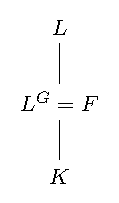
\includegraphics{lectures/5/pictures/cd_7.pdf}
		\end{center}

		где верхний этаж~--- расширение Галуа, а нижний~--- чисто несепарабельное расширение\footnote{Вообще говоря, в характеристике 0 такого возникать не может}. 

		Введём соответствующие кольца целых $\cO_{L} = \Int_{L}{A}$ и $\cO_{L} = \Int_{F}{A}$. Тогда у нас есть расширение 
		\begin{center}
			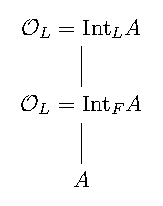
\includegraphics{lectures/5/pictures/cd_8.pdf}
		\end{center} 

		Так как расширение $L/F$ сепарабельно, $\cO_{F}$ целозамкнуто, мы можем применить теорему~\ref{B_is_finite_A_module} и получить, что $\cO_{L}$~--- конечнопорожденный $\cO_{F}$-модуль. 

		Далее, из общей теории полей следует, что чисто несепарабельное расширение устроено следующим образом: 
		\[
			F = \bk\lr*{ y^{\frac{1}{p^{m_1}}}, \ldots, y^{\frac{1}{p^{m_s}}} }, \text{ где } y_i \in A, \ p = \Char{\bk}.
		\]

		Тогда, если мы возьмём $m = \max{m_i}$, то мы получим
		\begin{equation}
			y_i = \sum a_I x^I \implies y_i^{\frac{1}{p^m}} = \sum a_I^{\frac{1}{p^m}} x^{I/p^m}, \label{eq_char_p}
		\end{equation}
		так как в характеристике $p$:
		\[
			\lr*{\sum a_I^{\frac{1}{p^{m}}} x^{\frac{I}{p^{m}}}}^{p^m}  = \sum \lr*{a_I^{\frac{1}{p^{m}}} x^{\frac{I}{p^{m}}}}^{p^m}
		\]
		а так как поле $\bk$ алгебраически замкнуто, $a^{\frac{1}{p^m}} \in \bk$. Но, из~\eqref{eq_char_p} следует, что 
		\[
			F \subset \bk\lr*{ x_1^{\frac{1}{p^m}}, \ldots, x_n^{\frac{1}{p^m}} }.
		\]
		Соответственно, если мы докажем теорему для $\bk\lr*{ x_1^{\frac{1}{p^m}}, \ldots, x_n^{\frac{1}{p^m}} }$, то мы докажем её и для $F$, так что далее без ограничений общности можно полагать, что 
		\[
			F = \bk\lr*{ x_1^{\frac{1}{p^m}}, \ldots, x_n^{\frac{1}{p^m}} }.
		\]

		Теперь покажем, что $\cO_{F} = \bk\left[ x_1^{\frac{1}{p^m}}, \ldots, x_n^{\frac{1}{p^m}} \right] = R$. Включение справа налево очевидно. Теперь пусть $\alpha \in \cO_{F}$, тогда $\alpha$ цел над $A$, значит он цел и над $R$, откуда $\alpha \in R$ (так как $R$ целозамкнуто и расширение $R/A$ конечно\footnote{Его базис состоит из мономов вида $x_1^{k_1/p^m} \cdot \ldots \cdot x_n^{k_n/p^m}$ по $0 \le k_i \le p^m - 1$}).

		Итак, мы показали, что $\cO_{F}/R$ конечно (а так как $R/A$ конечно и $\cO_L/\cO_F$ конечно), из этого следует теорема.


	 	\end{proof}

	 	\begin{definition} 
	 		Если в предыдущей теореме $L = K$, то $B$ называется \emph{нормализацией} $A$.
	 	\end{definition}

	 	\begin{remark}
	 		Отметим, что в этом случае $B$ является аффинной $\bk$-алгеброй. 
	 	\end{remark}

	 	\begin{definition} 
	 		Пусть $\varphi\colon Y \to X$~--- морфизм многообразий. Предположим, что у любой точки $x \in X$ есть такая аффинная окрестность $U_x$, что $\varphi^{-1}(U_x) \cong V_x$, где $V_x$~--- аффинная, и расширение $A(U_x) \hookrightarrow A(V_x)$ конечным. Тогда $\varphi$ называется \emph{конечным морфизмом}. 
	 	\end{definition}

	 	\begin{definition} 
	 		Пусть $X$~--- аффинное многообразие. Тогда $X$ называется \emph{нормальным}, если $X = \Specm(A)$, где $A$~--- нормальное.
	 	\end{definition}

	 	\begin{remark}
	 		Локализация нормального кольца нормальна. 
	 	\end{remark}

	 	\begin{definition} 
	 		Неприводимое многообразие $X$\footnote{Уже не обязательно аффинное} называют \emph{нормальным}, если $\forall P \in X$ кольцо $\cO_{P}$ нормально. 
	 	\end{definition}

	 	\begin{statement} 
	 		Предыдущие два определения нормальности согласованы.  
	 	\end{statement}
	 	\begin{proof}
	 		Нам нужно доказать следующее утверждение: если $\forall \fm \in \Specm(A)$ кольцо $A_{\fm}$ нормально, то $A$ нормально (для целостного кольца $A$).

	 		Покажем, что $A = \bigcap_{\fm \in \Specm(A)} A_{\fm}$. Действительно, включение слева направо очевидно, а если $x \in \bigcap_{\fm \in \Specm(A)} A_{\fm}$, то $\forall \fm \in \Specm(A)$ найдётся $y_{\fm} \notin \fm$ такой, что $xy_{\fm} \in A$. Тогда, так как никакой $y_{fm}$ не лежит ни в каком максимальном идеале, $(\{ y_{\fm}\}_{\fm})$~--- единичный идеал. Но тогда 
	 		\[
	 			1 = \sum y_{\fm} z_{\fm} \implies x = \sum_{} x y_{\fm} z_{\fm} \in A.
	 		\]
	 		Тогда, так как каждое кольцо в правой части целозамкнуто, и само $A$ целозамкнуто. 
	 	\end{proof}

	 	
	 	